\documentclass[parskip=full,11pt,twoside]{scrartcl}
\usepackage[utf8]{inputenc}

\title{ATURL: Actually Tiny URLs}
\author{Kaylee Frye, Derrial Book}

% section numbers in margins:
\renewcommand\sectionlinesformat[4]{\makebox[0pt][r]{#3}#4}

% header & footer
\usepackage{scrlayer-scrpage}
\lofoot{\today}
\refoot{\today}
\pagestyle{scrheadings}

\usepackage[sfdefault,light]{roboto}
\usepackage[T1]{fontenc}
\usepackage[german]{babel}
\usepackage[yyyymmdd]{datetime} % must be after babel
\renewcommand{\dateseparator}{-} % ISO8601 date format
\usepackage{hyperref}
\usepackage[nameinlink]{cleveref}
\crefname{figure}{Abb}{Abb}
\usepackage[section]{placeins}
\usepackage{xcolor}
\usepackage{graphicx}
\hypersetup{
	pdftitle={Pflichtenheft},
	bookmarks=true,
}
\usepackage{csquotes}

\usepackage{amsmath} % for $\text{}$
\newcommand\urlpart[2]{$\underbrace{\text{\texttt{#1}}}_{\text{#2}}$}

\usepackage{pflichtenheft}

\begin{document}
\maketitle

\section{Einleitung}

Das Universum braucht einen besseren URL Shortener.

URL Shortening erzeugt kurze URLs,
die nur Weiterleitungen sind zu sehr viel längeren URLs.
Das ist nützlich, weil Kurz-URLs besser zu merken sind
und leichter mündlich weiterzugeben.
Ebenfalls nützlich sind sie,
wenn URLs im Text auftauchen (bspw. IRC).

Eine URL besteht aus mehreren Komponenten:

\begin{center}
\urlpart{http}{protocol}%
\texttt{://}%
\urlpart{web.io}{host}%
\texttt{/}%
\urlpart{index}{path}%
\texttt{?}%
\urlpart{argument=somevalue}{parameter}%
\texttt{\#}%
\urlpart{theAnchor}{fragment}
\end{center}

Für Kurz-URLs ist der path (engl.\ Pfad) relevant.
Das Protokoll ist HTTP oder HTTPS, abhängig vom Besucher.
Die Wahl des host-Namens ist nicht Teil der Softwareentwicklung,
sondern des Betreibers.
Parameter und Fragment werden nicht genutzt,
da es mindestens einen zusätzlichen Buchstaben braucht
und damit die URL verlängert.

Im weiteren Text nehmen wir an,
dass der Dienst unter dem Hostnamen \texttt{atu.rl} angeboten wird.

\pagebreak
\section{Kriterien}
% Diese Section sollte kurz und knapp "für Manager" sein
% und auf eine Seite passen.

\subsection{Muss}

\criterium{Beschränkte Länge}{crt:length}

Der Pfad von Kurz-URLs ist exakt 3 ASCII Buchstaben oder Ziffern lang.
Das beschränkt die Anzahl der möglichen URLs auf knapp 200.000 Kurz-URLs.

\criterium{Schnelle Weiterleitung Kurz- zu Lang-URL}{crt:fast}

\criterium{Authentifizieren mit E-Mail oder Facebook}{crt:login}

\criterium{Rechtlichte Vorgaben werden eingehalten}{crt:tmg}

Der Dienst befolgt alle in Deutschland geltenden Richtlinien,
insbesondere das Telemediengesetz.

\subsection{Kann}

\criteriumOptional{Authentifizieren mit Github}{crt:github}

\criteriumOptional{Seite mit Betreiberinfo}{crt:about}

Der Dienst bietet eine Seite \enquote{Über Uns},
mit Informationen zum Betreiber.

\subsection{Abgrenzung}

\criteriumNot{Keine Wahl Kurz-URL}{crt:no-choice}

Ein Nutzer hat keine Möglichkeit die Auswahl einer Kurz-URL zu beeinflussen.

\pagebreak
%%%%%%%%%%%%%%
\section{Produkteinsatz}

Das Produkt soll mit minimalen Administrationskenntnissen zu betreiben sein.

Besucher des Diensts sollen diesen ohne Schulung oder andere Information benutzen können.

\section{Produktumgebung}

Das Programm soll als Servlet in einem Apache Tomcat betrieben werden.

Es stehen mindestens 2 AMD64 Kerne mit insgesamt 2GB shared RAM zur Verfügung.

%%%%%%%%%%%
\section{Funktionale Anforderungen}

\functionality{Schnelle Weiterleitung}{fnc:o1}
\fulfills{crt:fast}

Um zu einer Kurz- die Lang-URLs zu finden,
benutzt der Dienst einen $O(1)$ Mechanismus.
Es wird sichergestellt,
dass mit einer zunehmenden Anzahl von Kurz-URLs im System
das Finden nicht länger dauert.

\functionality{Login-Möglichkeit auf Homepage}{fnc:login}
\fulfills{crt:login}
\fulfills{crt:github}

Auf der Homepage \texttt{http://atu.rl/} sieht ein Besucher
einen \enquote{Login via Facebook} Knopf.
Weitere Knöpfe wie \enquote{Login via Github} sind möglich.
Siehe \cref{fig:homepage}.

\functionality{Auf jeder Seite ist ein Link \enquote{Impressum}}{fnc:impressum-link}
\fulfills{crt:tmg}

Entsprechend Telemediengesetz (TMG) §1
müssen gewisse Informationen über einen Betreiber jederzeit verfügbar sein.
Die inzwischen etablierte Vorgehensweise ist auf allen~(!) Seiten
einen Link mit dem Text \enquote{Impressum} anzubieten.
Dieser Link für auf eine Seite mit entsprechender Erklärung.

\functionality{Auf jeder Seite ist ein Link \enquote{Datenschutz}}{fnc:datenschutz-link}
\fulfills{crt:tmg}

Entsprechend Telemediengesetz (TMG) §13
muss der Betreiber den Nutzer Speicherung und Verarbeitung seiner personenbezogenen Daten unterrichten.
Die inzwischen etablierte Vorgehensweise ist auf allen (!) Seiten
einen Link mit dem Text \enquote{Datenschutz} anzubieten.
Dieser Link für auf eine Seite mit entsprechender Erklärung.

\functionality{Daten werden persistent gespeichert}{fnc:persistence}

Ein geordneter Neustart des Diensts führt nicht zu Datenverlust.

%%%%%%%%%%%
\section{Nicht-Funktionale Anforderungen}

\nonFunctionality{Modernes Design}{nfc:design}

Das Design soll modern und seriös wirken.

\nonFunctionality{Persistenz}{nfc:persistence}

Sollten in Zukunft Erweiterungen oder Updates notwendig werden,
müssen die Daten (Kurz-URLs, E-Mailaddressen) erhalten bleiben.

\nonFunctionality{Erweiterbarkeit}{nfc:extensibility}

Das Produkt muss dahingehend erweiterbar sein,
das die Liste der E-Mail-URL Abbildung von authentifizierten Nutzern
abgerufen werden kann.
Wie das genau implementiert wird, ist nicht Teil dieses Projekts.

%%%%%%%%%%%
\section{Tests}

\test{Kurz-URL Erstellen}{tst:create}
\tests{fnc:login}

\teststep{Besucher \enquote{Zoe Washburne} hat einen Browser geöffnet.}
{Zoe navigiert auf die Homepage \texttt{http://atu.rl/}.}
{Die Homepage wird angezeigt wie in \cref{fig:homepage}.}

\teststep{Zoe hat einen Facebook-Account.}%
{Zoe drückt den \enquote{Login via Facebook} Knopf.}%
{Zoe wird eingeloggt und auf die Erstellseite wie in \cref{fig:form} weitergeleitet.}

\teststep{}
{Zoe befüllt das Feld \enquote{URL} mit \texttt{sehrlangedomain.com/undganzlangeURL.html} und drückt auf \enquote{Kurz-URL erstellen}.}%
{Ihr wird eine Kurz-URL angezeigt wie z.B.\ \texttt{atu.rl/abc}
 wie in \cref{fig:generated}.
 Statt \enquote{abc}, dürfen beliebige andere Buchstaben und Zahl angezeigt werden, allerdings exakt drei.}

\teststep{}
{Zoe navigiert auf die eben generierte Kurz-URL, z.B.\ \texttt{http://atu.rl/abc}.}
{Sie wird zu \texttt{sehrlangedomain.com/undganzlang  eURL.html} weitergeleitet.}

\test{Betreiberinfos lesen}{tst:tmg}
\tests{fnc:impressum-link}
\tests{fnc:datenschutz-link}

\teststep{Besucher \enquote{Jayne Cobb} ist auf der Homepage}
{Er folgt dem Link mit dem Text \enquote{Datenschutz}}
{Ein Text mit allen Datenschutzinformationen wird ihm angezeigt.}

\teststep{}
{Jayne folgt dem Link mit dem Text \enquote{Impressum}}
{Ein Text mit Informationen des Betreibers wird ihm angezeigt.}

%%%%%%%%%%%%%
\pagebreak
\appendix

\section{Seitenentwürfe}

% made via https://gomockingbird.com/projects/mnf0cwf/4gXVnC

\begin{figure}[hb]
\fbox{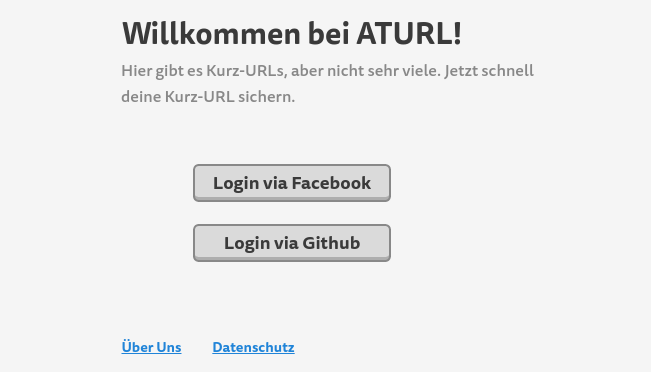
\includegraphics[width=\textwidth]{image/login.png}}
\caption{\label{fig:homepage}
Homepage mit Login-Funktion
}
\end{figure}

\begin{figure}[hb]
\fbox{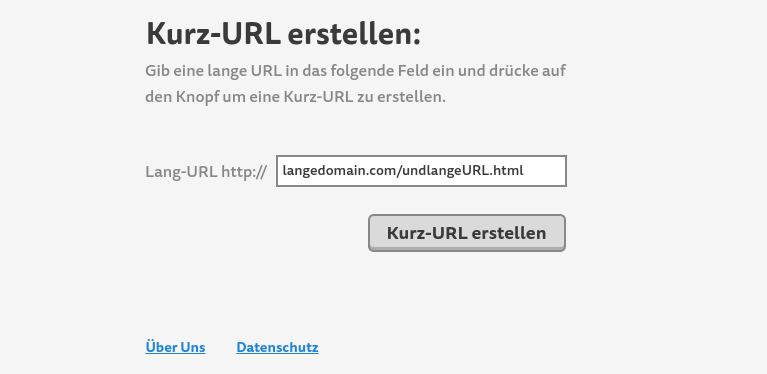
\includegraphics[width=\textwidth]{image/form.png}}
\caption{\label{fig:form}
Formular zur Generierung einer Kurz-URL.
Getestet beispielsweise in \testlink{tst:create}.
}
\end{figure}

\begin{figure}[hb]
\fbox{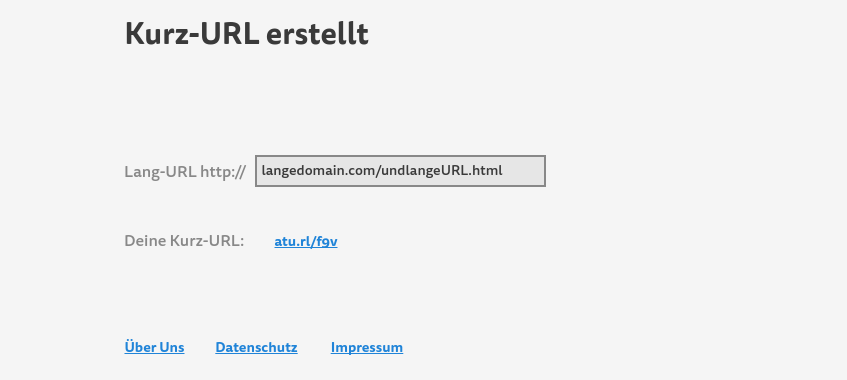
\includegraphics[width=\textwidth]{image/generated.png}}
\caption{\label{fig:generated}
Anzeige der generierten Kurz-URL.
Das Textfeld mit der Lang-URL kann nicht geändert werden.
}
\end{figure}

\section{Glossar}

\textbf{Besucher}:
Eine Person, welche den Dienst nutzt.
Kann eingeloggt sein oder nicht.

\textbf{Dienst}:
Die Software im laufenden Betrieb. Software as a Service.

\textbf{Homepage}:
Seite, die beim Besuchen der Betreiberdomain \emph{ohne Pfad} angezeigt wird. Auch \enquote{Startseite}.

\textbf{Nutzer}:
Ein eingeloggter Besucher.

\end{document}
